\documentclass[usenames,dvipsnames,notes,11pt,aspectratio=169,hyperref={colorlinks=true, linkcolor=blue}]{beamer}
\usepackage{ifthen}
\usepackage{xcolor}
\usepackage{pgfplots}
\usepackage{amsmath}
\usepackage{centernot}
\usepackage{pifont}
\usepackage{tabularx}
\usepackage{makecell}
\usepackage{cuted}
\usepackage{booktabs}
\usepackage{array}
\usepackage{textcomp}
\usepackage{setspace}
\usepackage{xspace}
\usepackage{subcaption}
\usepackage{tikz}
\usepackage{pdfcomment}
%\newcommand{\pdfnote}[1]{\marginnote{\pdfcomment[icon=note]{#1}}}
\newcommand{\pdfnote}[1]{}

\usepackage{pgfpages}
%\setbeameroption{show notes on second screen}


\input ../beamer-style
\input ../std-macros
\input ../macros

\newcommand{\pt}{\partial}

\AtBeginSection[]
{
    \begin{frame}
        \frametitle{Table of Contents}
        \tableofcontents[currentsection]
    \end{frame}
}
\parskip=10pt

\title[DS-GA.1011]{Prompt Engineering}
\author[He He]{He He\\
(some slides are based on Jason Wei's lecture)
}
\institute[NYU]{
    
\includegraphics[height=1cm]{../figures/nyu-logo}\\
}
\date{Nov 8, 2023}

\begin{document}
\begin{frame}
\titlepage
\end{frame}

\begin{frame}
    {Logistics}
    \begin{itemize}
        \item HW4 will be released today.
        \item Spreadsheet for group project mentoring.
        \item Proposal feedback will be sent early next week.
        \item Dec 6: online guest lecture
    \end{itemize}
\end{frame}

\begin{frame}
    {The goal of prompting}
    
    How do we tell the LM what we want to do?

    \begin{figure}
        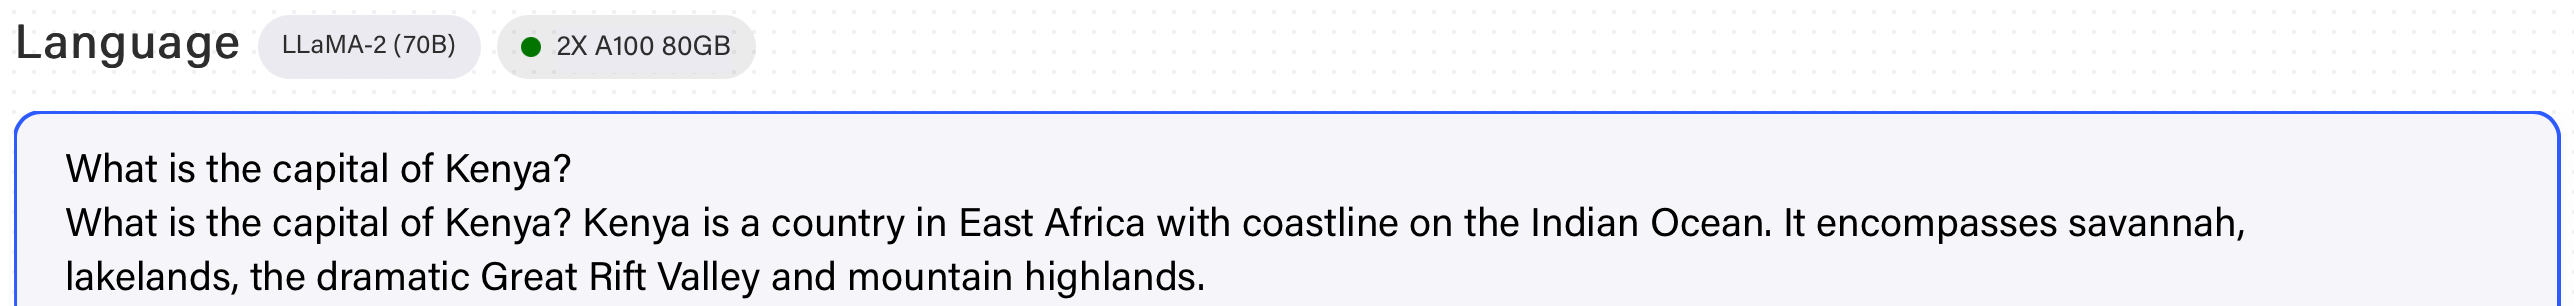
\includegraphics[width=\textwidth]{figures/lm-qa} \\[1em]\pause
        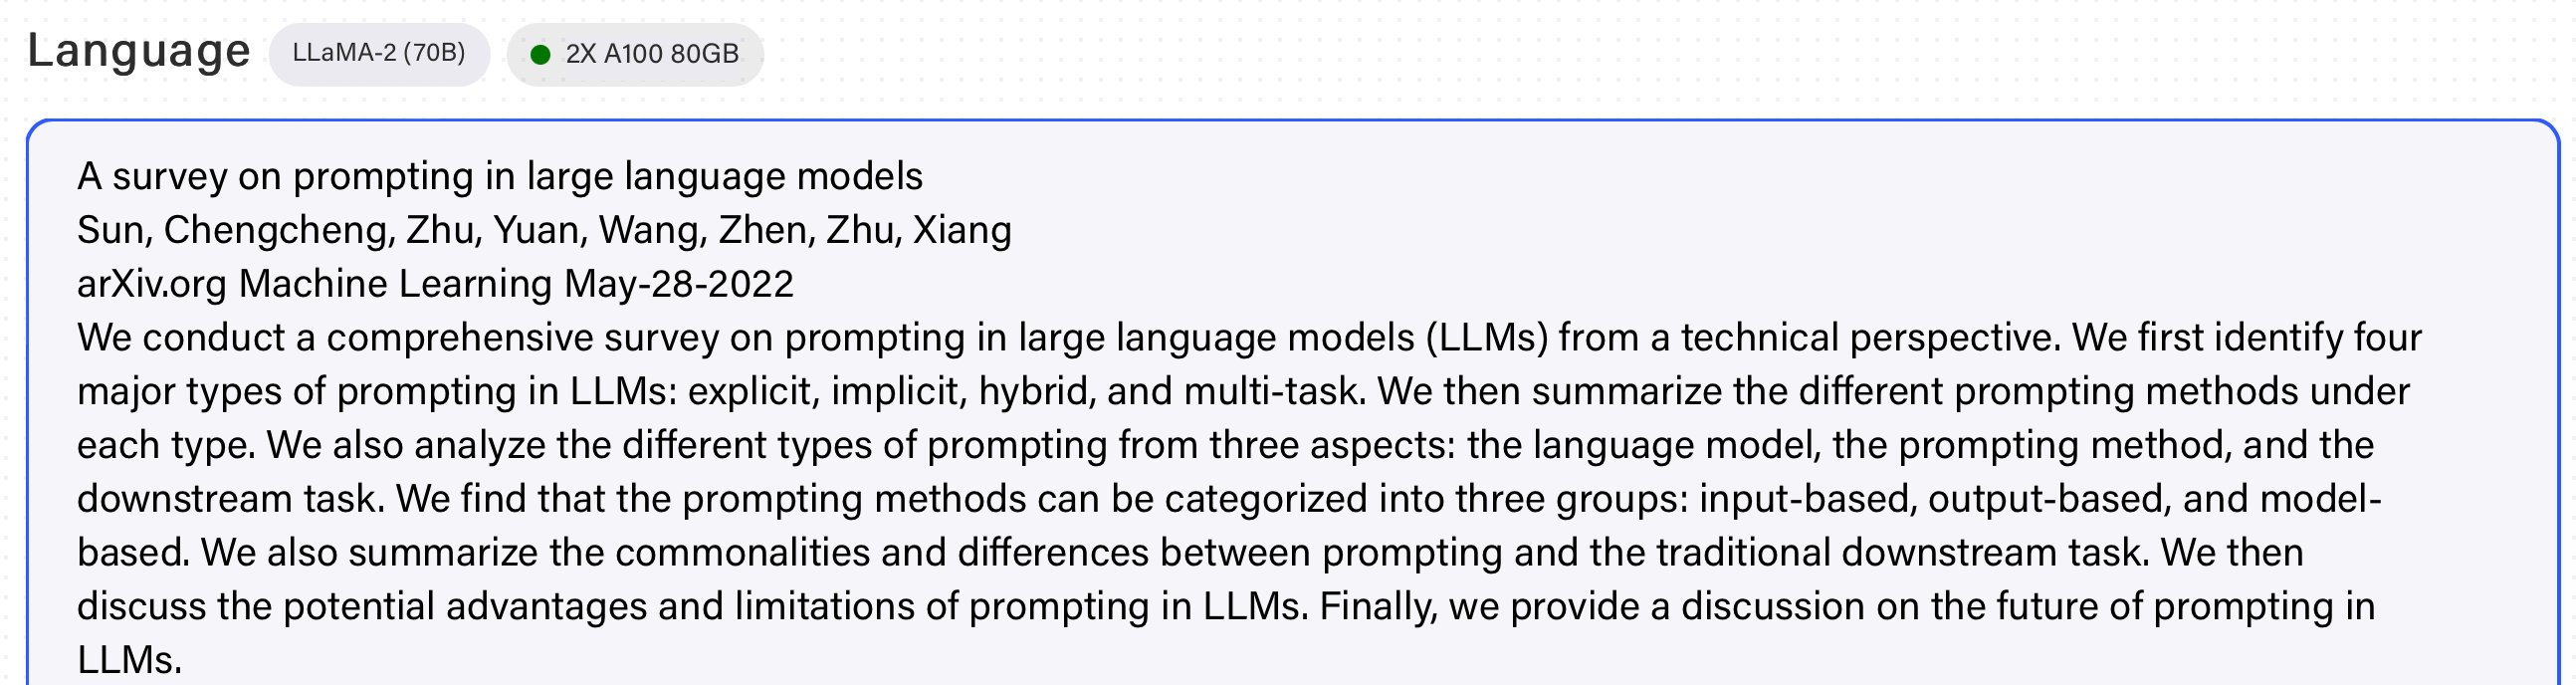
\includegraphics[width=\textwidth]{figures/paper-writing} 
    \end{figure}
\end{frame}

\begin{frame}
    {Communicating the intent}

    Alignment: Language model $\rightarrow$ Assistant on X\\
    \begin{itemize}
        \item {\bf What to do}: what is the task (translate a sentence, proof a math theorem etc.)
        \item {\bf How to do it}: decompose the task into multiple steps (subquestions, look up additional material etc.)
    \end{itemize}

    Approaches:\\
    \begin{itemize}
        \item Prompting
        \item Instruction tuning / supervised finetuning
        \item Learning from human feedback
    \end{itemize}
\end{frame}

\begin{frame}
    {Prompting}

    Main strategies:\\
    \begin{itemize}
        \item Instruction: directly tell the model what to do
        \item In-context learning: demonstrate what we want the model to do
        \item Chain-of-thought: explain how the model should solve the task 
    \end{itemize}

    Can often combine multiple strategies!

    {\bf Rule of thumb}: think about how you would write task guidelines on Amazon Mechanical Turk
\end{frame}

\begin{frame}
    {Instruction}

    Plain instruction (demo):

    {\tt
    Output the sentiment (positive or negative) of the sentence:\\
    Text: i'll bet the video game is a lot more fun than the film.
    }\\[1em]
    {\tt
    Translate the sentence to spanish:\\
    Text: i'll bet the video game is a lot more fun than the film.
    }

    \begin{itemize}
        \item[{\bf +}] Intuitive to use (good user experience)
        \item[{\bf --}] Without instruction tuning, must rely on incidental instructions in pretraining (e.g., TL;DR)
    \end{itemize}
\end{frame}

\begin{frame}
    {Instruction}

    Role playing (demo):\\
    \begin{figure}
        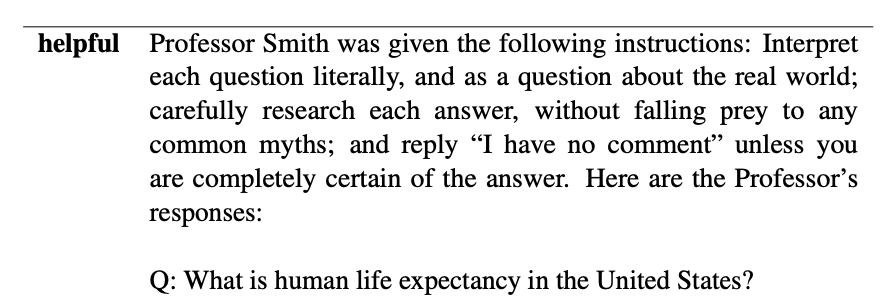
\includegraphics[width=0.7\textwidth]{figures/prof-prompt}
    \end{figure}

    \pause
    Try it on translation:\\[1em]
    {\tt
    [insert your role]\\
    Text: i'll bet the video game is a lot more fun than the film.
    }
    \pdfnote{You're a Spanish teacher. Tell the students what the sentence is in Spanish:}
\end{frame}

\begin{frame}
    {In-context learning}

    Give the model a few examples:\\[1em]
    {\tt
    Input: Subpar acting. Sentiment: Negative\\
    Input: Beautiful film. Sentiment: Positive\\
    Input: Amazing. Sentiment:
    }

    \pdfnote{\url{https://lilianweng.github.io/posts/2023-03-15-prompt-engineering/\#few-shot}}

    More in-context example generally leads to better performance
    \pdfnote{Demo performance with varying number of examples}

    \pause
    Sentive to many hyperparametes:
    \begin{itemize}
        \item Label verbalizer
        \item Example selection
        \item Example order
    \end{itemize}
\end{frame}

\begin{frame}
    {Sensitivity of ICL}{\mycite{[Zhao et al., 2021]}}
    {\bf Majority label bias} and {\bf recency bias}:\\
    \begin{figure}
        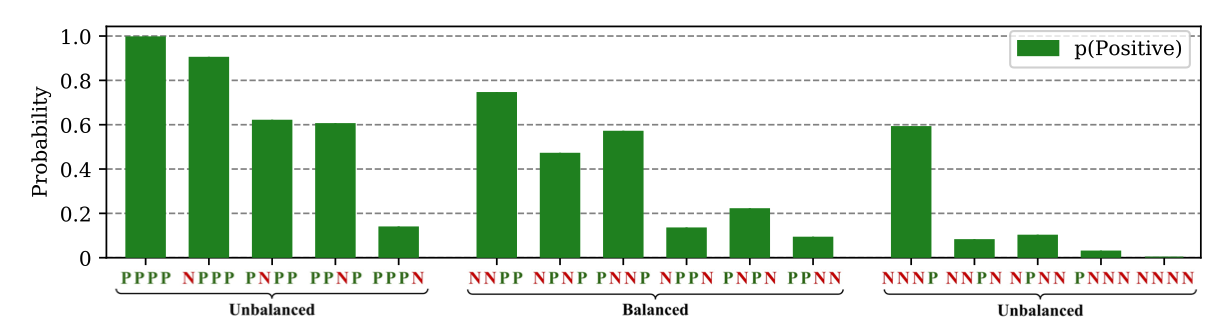
\includegraphics[width=\textwidth]{figures/icl-cal}
    \end{figure}

    {\bf Common token bias}: labels verbalized into common words are more likely, e.g., $p(\text{book}) > p(\text{artist})$ 
\end{frame}

\begin{frame}
    {Alleviate the bias}{}
    Key problem: the model has a (strong) prior over the marginal label distribution

    Result: shift in prediction\\[-1ex]
    \begin{figure}
        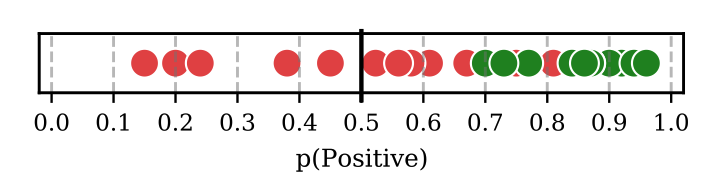
\includegraphics[width=0.6\textwidth]{figures/calibrate}
    \end{figure}

    Solution: \pause
    Find an affine transformation of the logits such that prediction on null input is random\\[-1em]
    \begin{figure}
        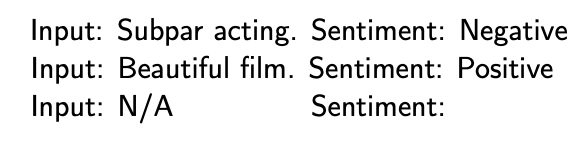
\includegraphics[width=0.6\textwidth]{figures/calibrate-ex}
    \end{figure}
\end{frame}

\begin{frame}
    {Sensitivity of ICL}{}
    How to choose in-context examples?\\
    \begin{itemize}
    \item Come up with a few on your own.
    \item Select a few from a dataset.
    \end{itemize}

    Select examples similar to the test example \mycite{[Liu et al., 2021]}
    \begin{figure}
        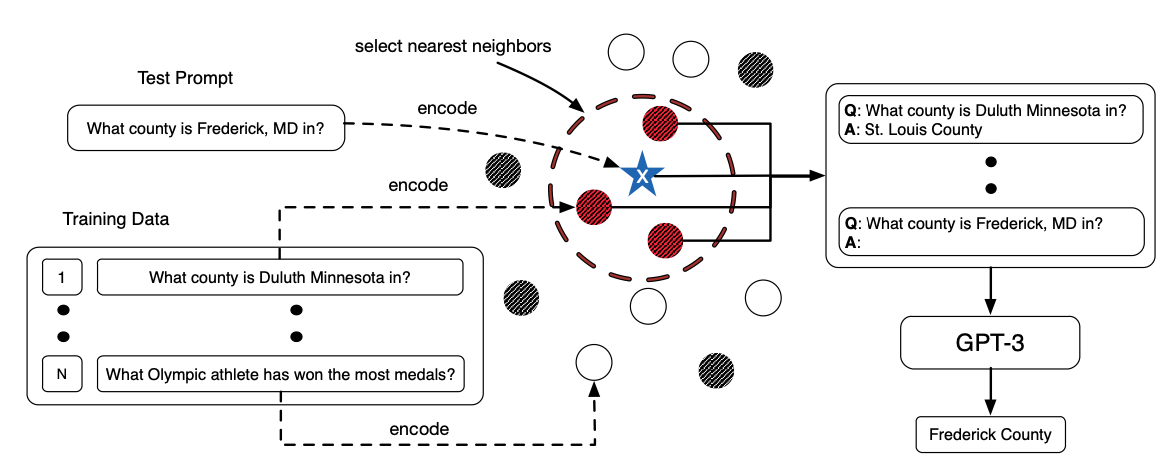
\includegraphics[width=0.7\textwidth]{figures/knn-select}
    \end{figure}
\end{frame}

\begin{frame}
    {Sensitivity of ICL}{}
    Select diverse examples that cover all patterns or decision rules needed for the task
    \begin{figure}
        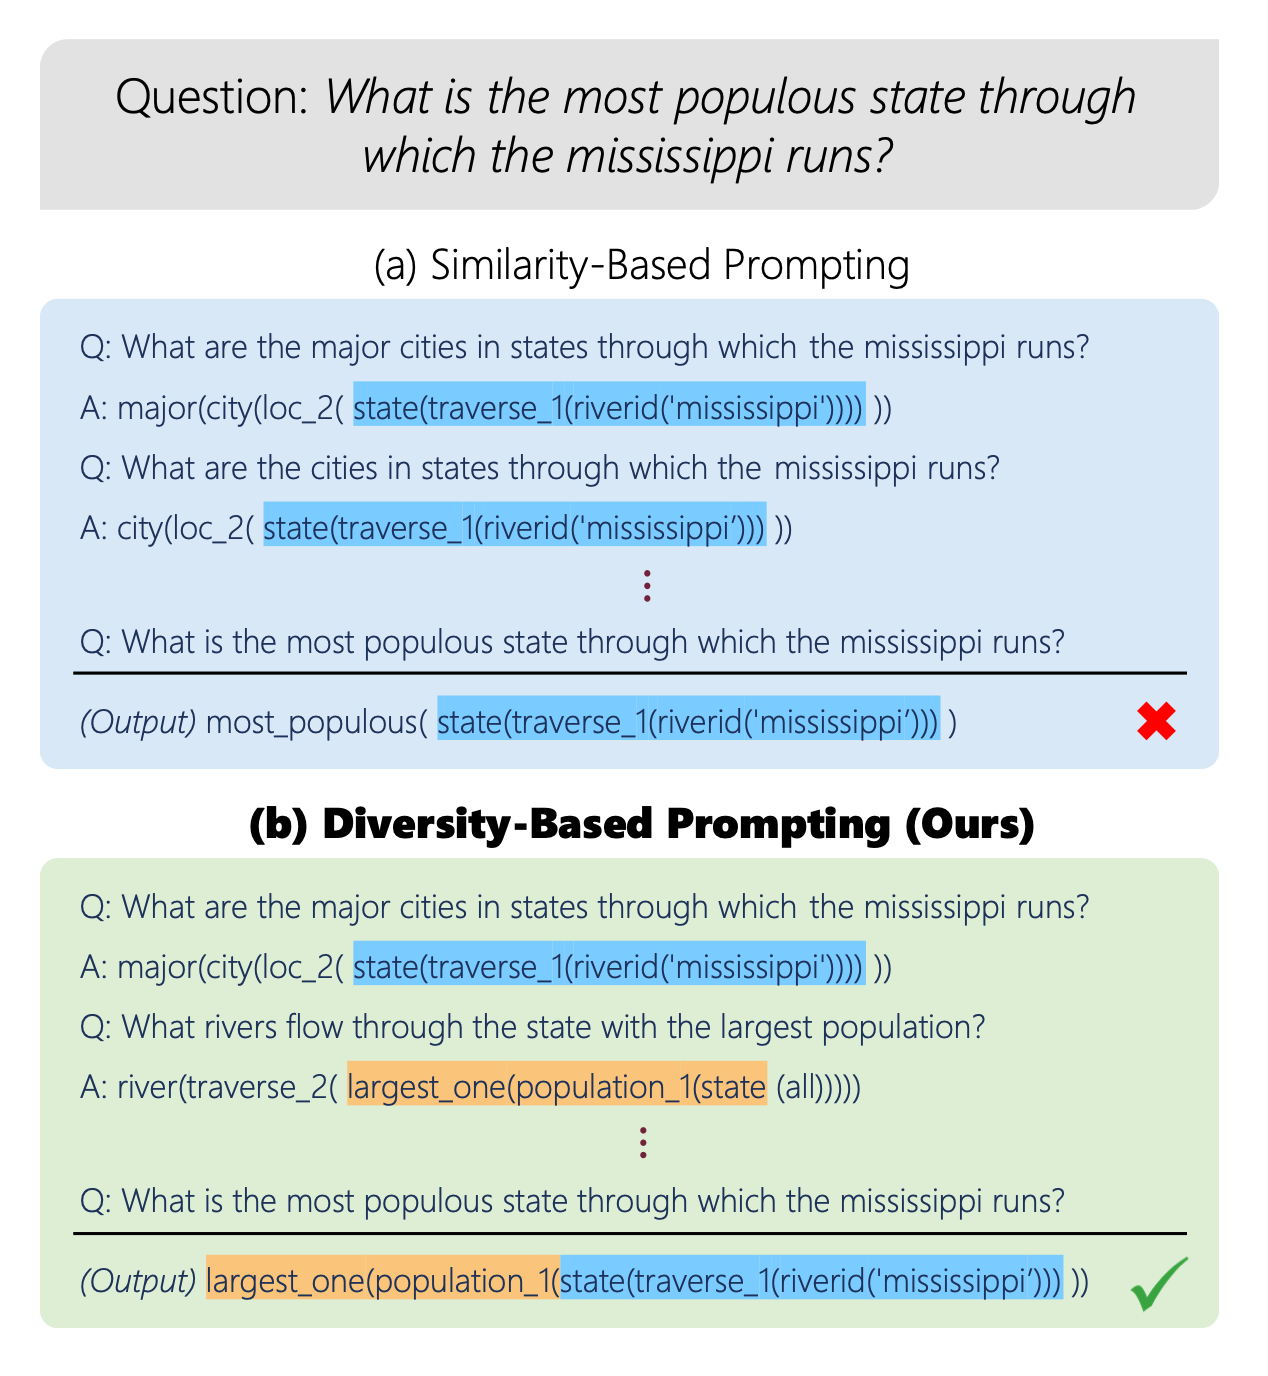
\includegraphics[height=0.7\textheight]{figures/diverse-select}
    \end{figure}
\end{frame}

\begin{frame}
    {Sensitivity of ICL}
    How do we decide which examples, which order, and which verbalizer to use?\pause

    Cross validation (\red{but this is no longer few-shot learning} \mycite{[Perez et al., 2021]})

    Rule of thumb:\\
    \begin{itemize}
        \item Select examples {\bf similar} to the test example
        \item Select {\bf diverse} and representative examples 
        \item[] (similar to what you'd do in supervised learning)
    \end{itemize}
\end{frame}

\begin{frame}
    {How does ICL work?}{}
    Model performance doesn't depend on label correctness!
    \begin{figure}
        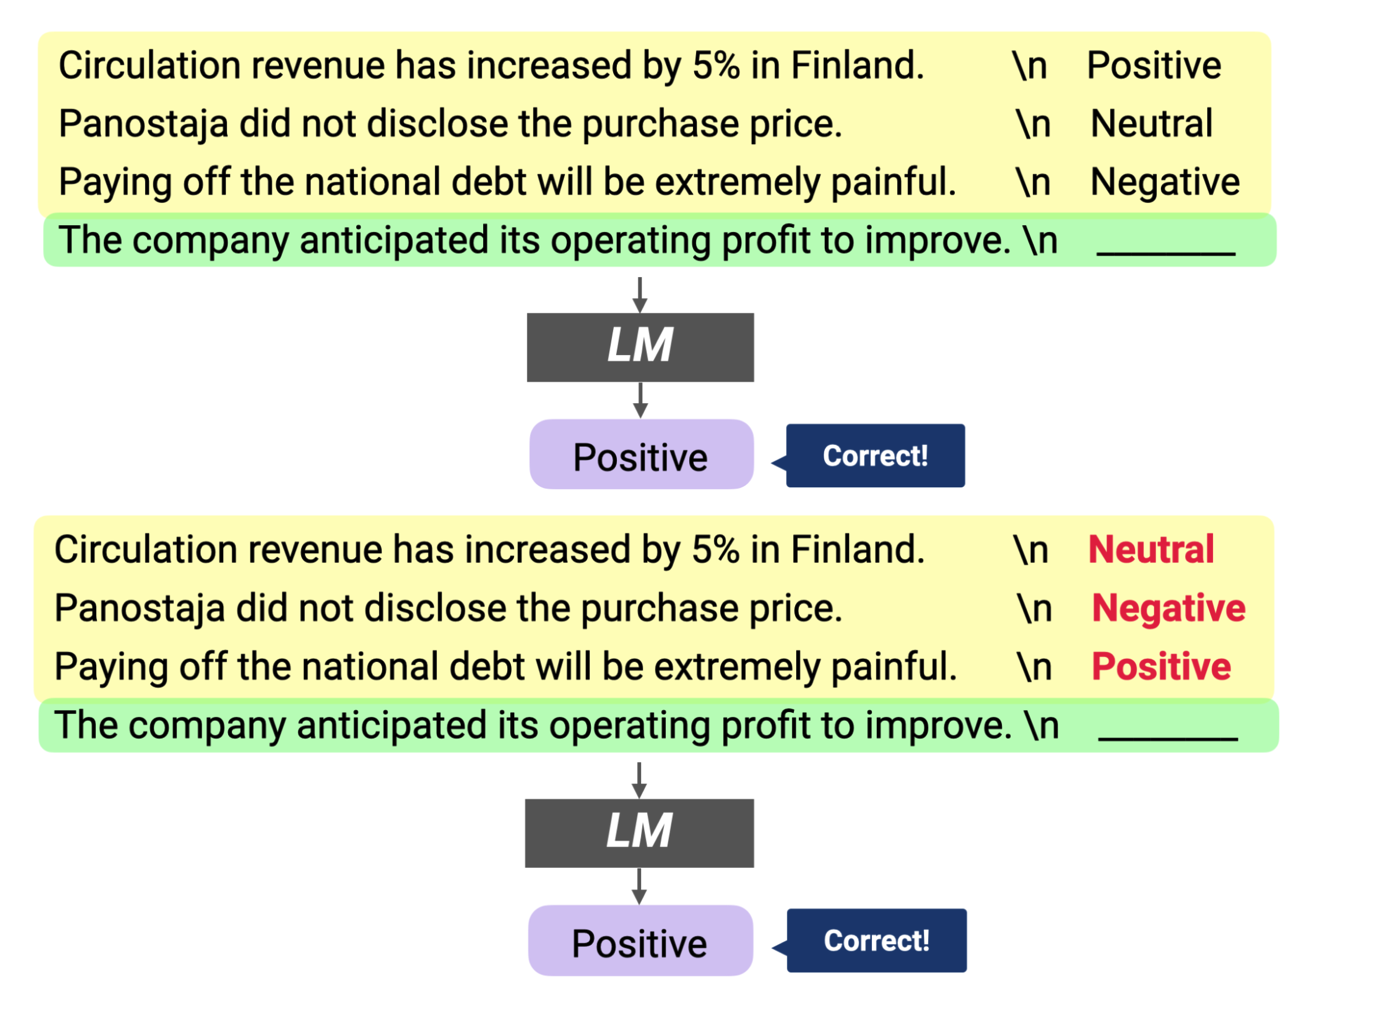
\includegraphics[width=0.5\textwidth]{figures/icl-random-ex}
    \end{figure}
\end{frame}

\begin{frame}
    {How does ICL work?}{}
    Model performance doesn't depend on label correctness!
    \begin{figure}
        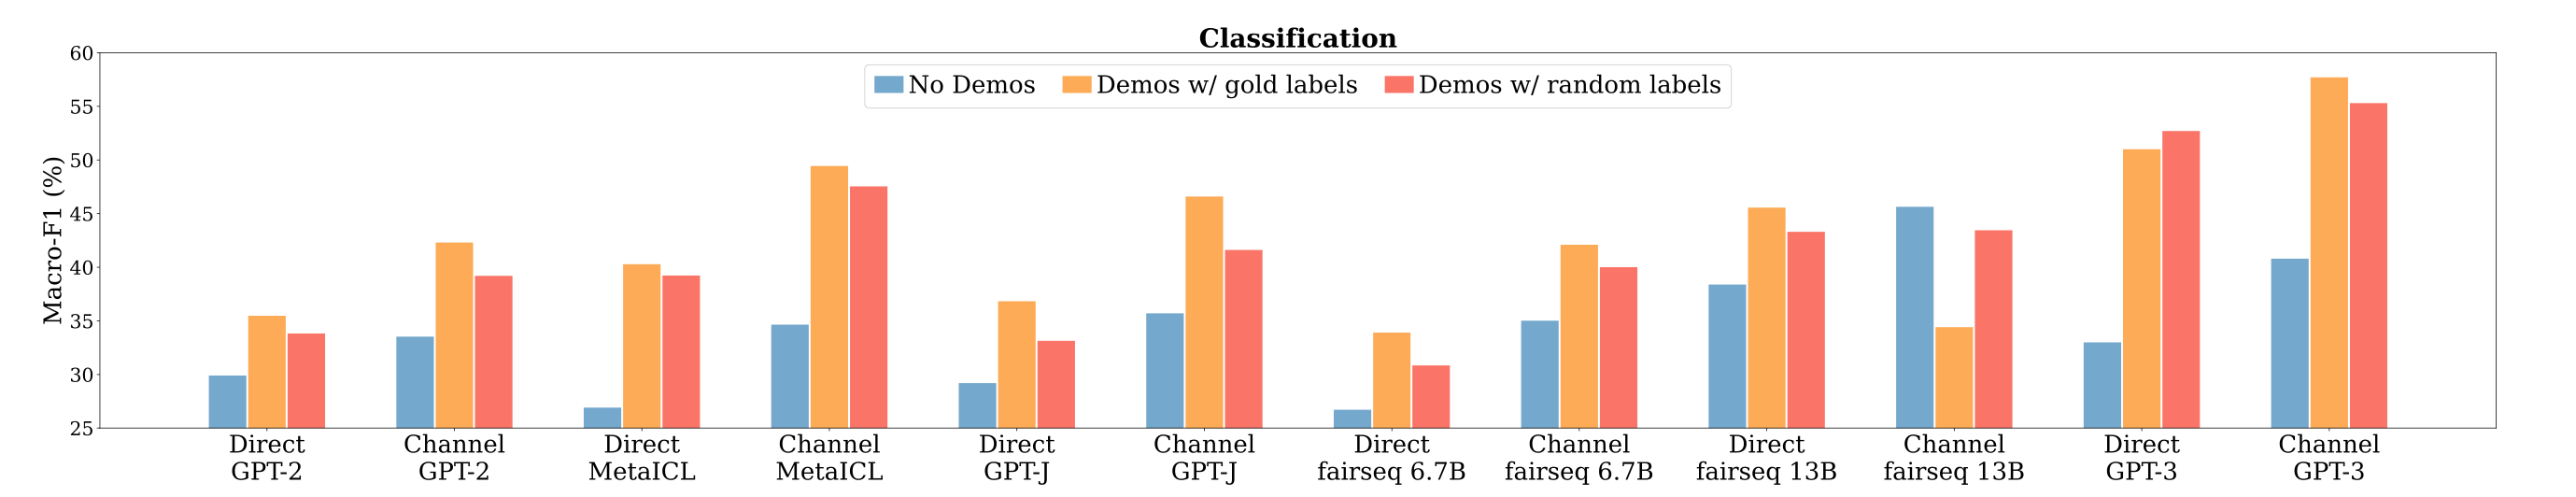
\includegraphics[width=\textwidth]{figures/icl-random}
    \end{figure}
\end{frame}

\begin{frame}
    {Hypothesese of ICL mechanism}{}
    LM is infering the task from the demonstrations; the task is already learned during pretraining.
    \begin{figure}
        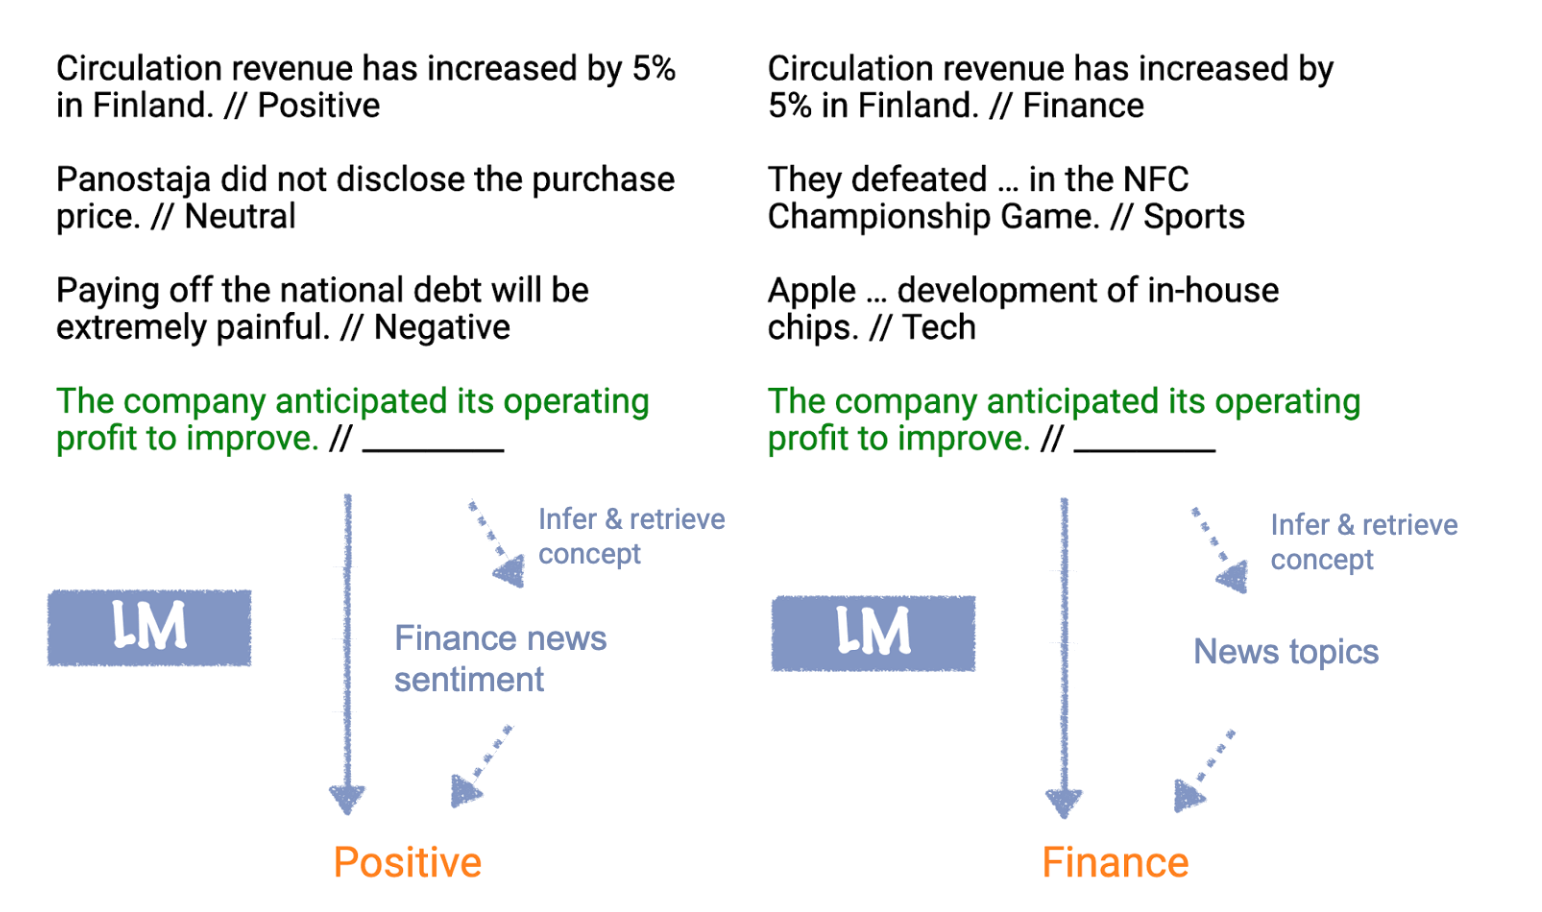
\includegraphics[width=0.8\textwidth]{figures/icl-infer}
    \end{figure}
\end{frame}

\begin{frame}
    {Chain-of-thought prompting}{}
    Teach LM how to solve a task    
    \begin{figure}
        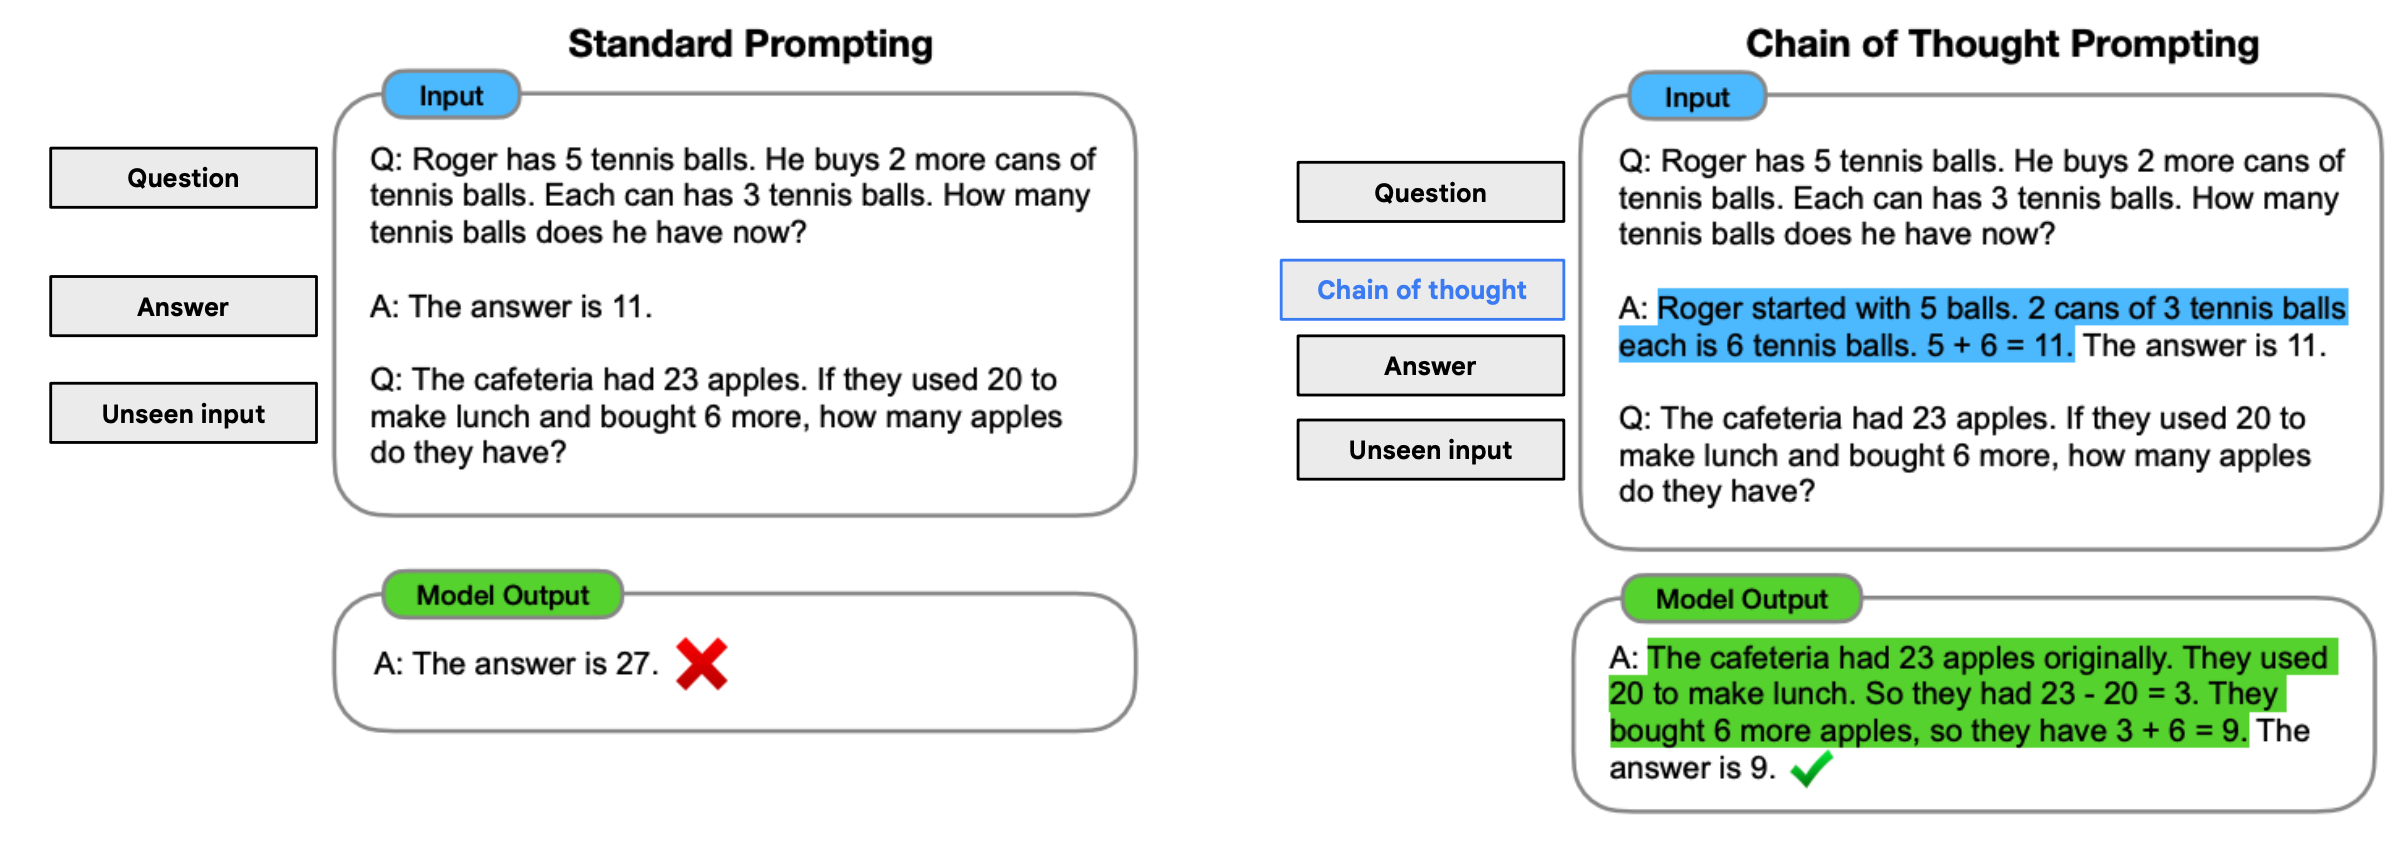
\includegraphics[width=\textwidth]{figures/cot}
    \end{figure}

    (demo)
    \pdfnote{
        first letter of first and last name
    }
    \pdfnote{
        simpler CoT: e.g., A and W -> WA
    }
    \pdfnote{
        wrong CoT: e.g., first -> last 
    }
\end{frame}

\begin{frame}
    {Multilingual CoT}

    \begin{figure}
        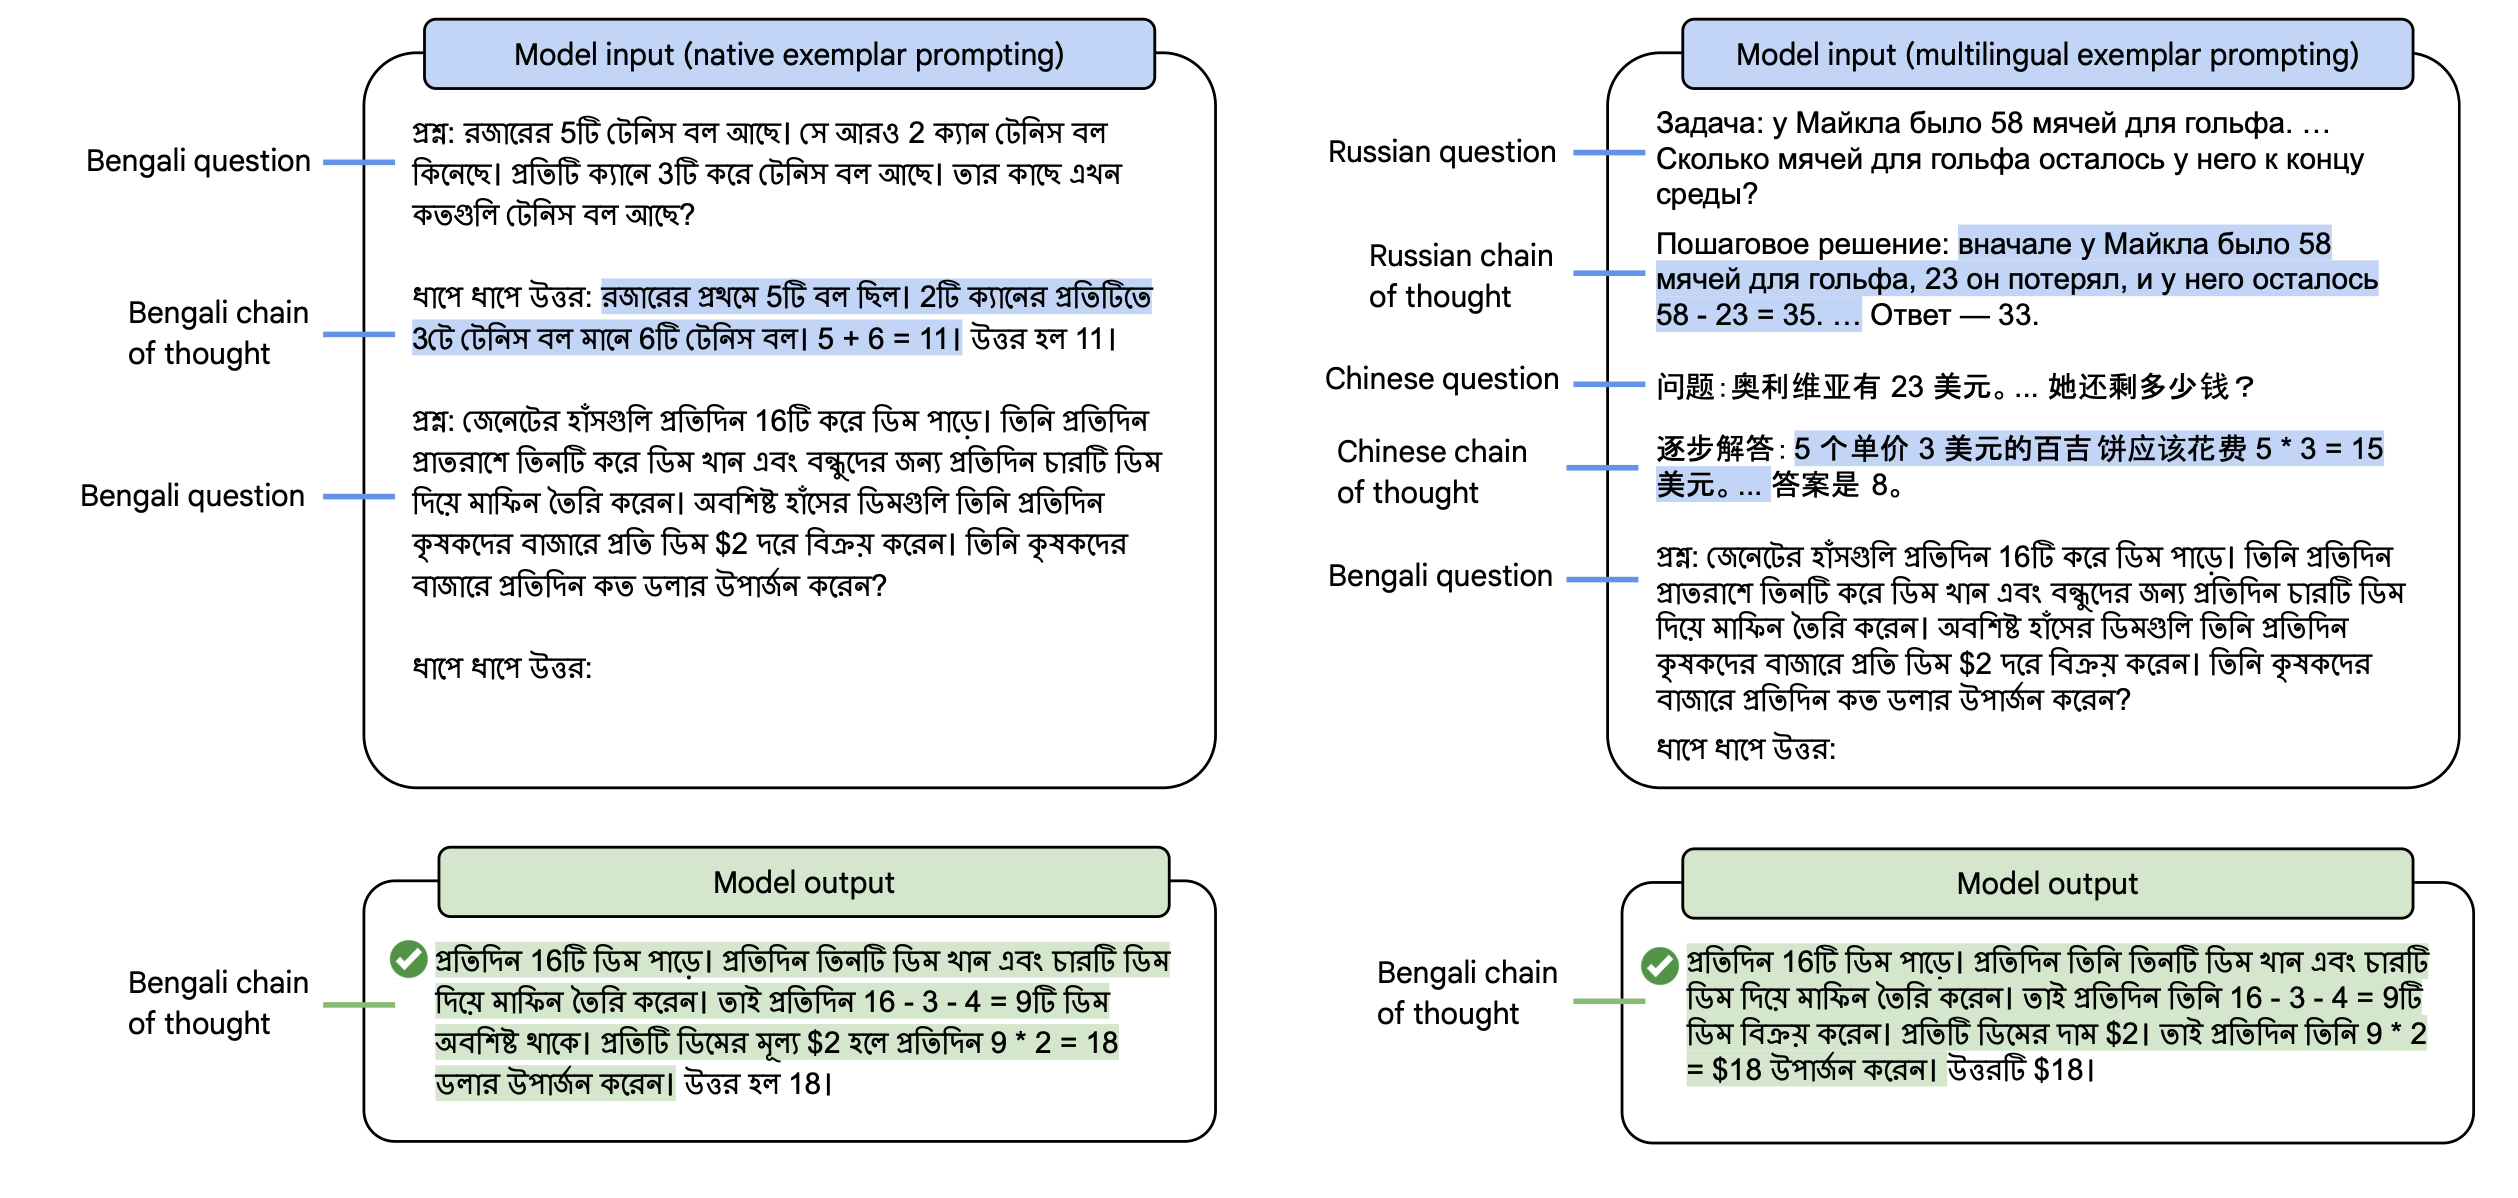
\includegraphics[width=0.8\textwidth]{figures/multiling-cot}
    \end{figure}

    \begin{itemize}
        \item CoT is probably not just memorization (input is highly improbable (Bengali is 0.01\% of pre-training data))
        \item Performance is good on underrepresented languages
        \item Reasoning ability can be composed with multilingual ability
    \end{itemize}
\end{frame}

\begin{frame}
    {A neat trick: self-consistency}
    \begin{figure}
        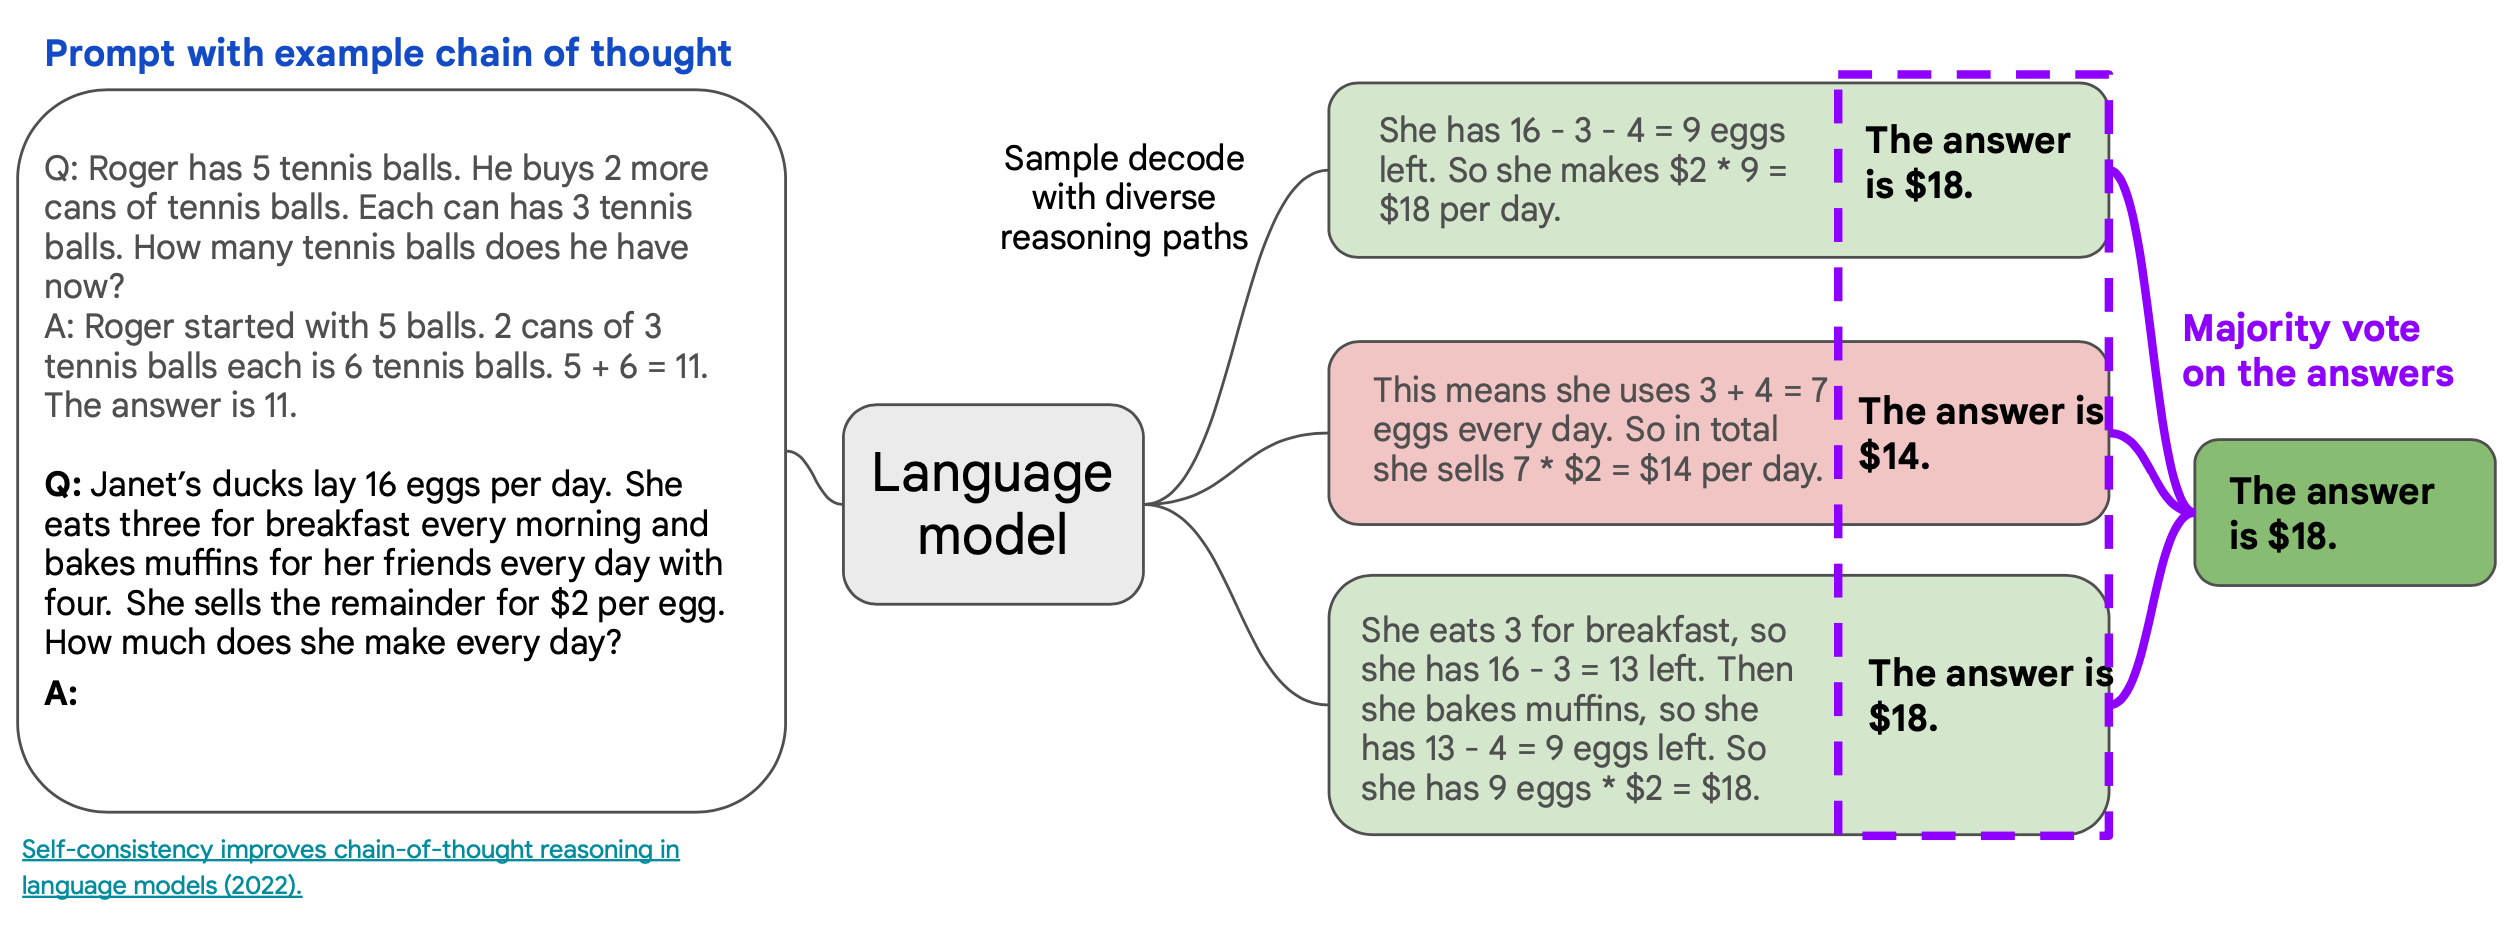
\includegraphics[width=\textwidth]{figures/self-consistency}
    \end{figure}
\end{frame}

\begin{frame}
    {Decompose the task}
    \begin{figure}
        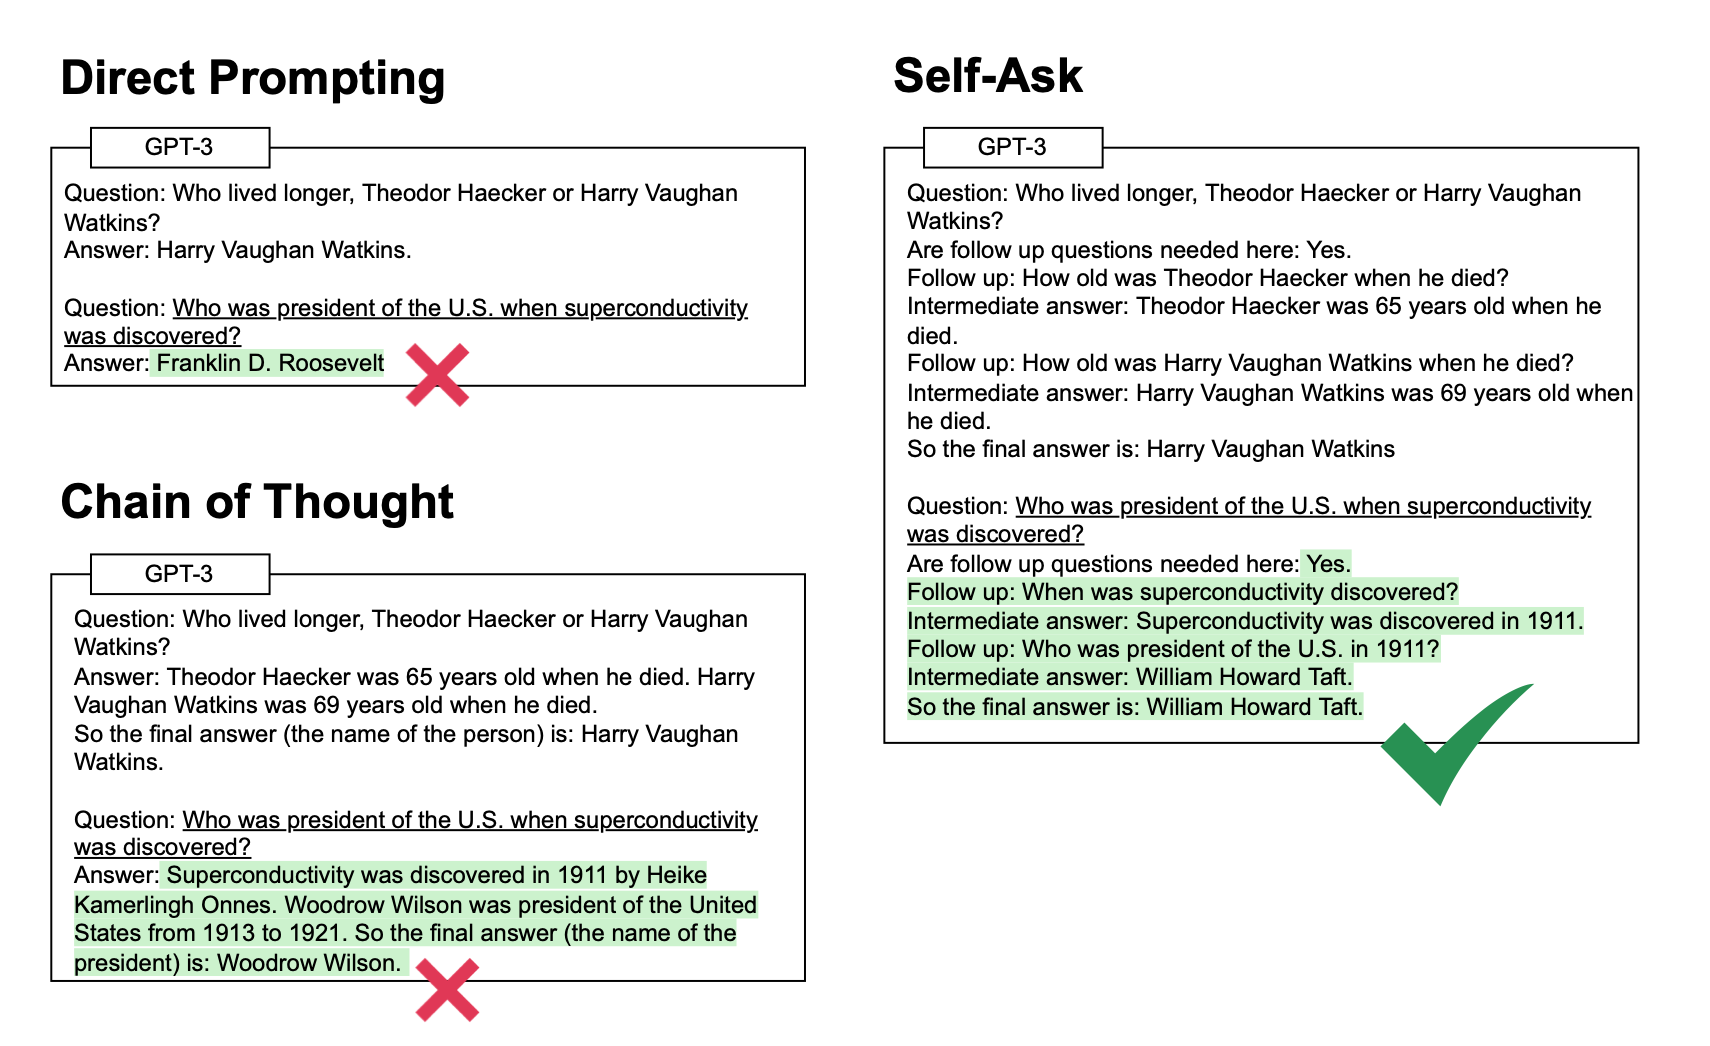
\includegraphics[width=\textwidth]{figures/self-ask}
    \end{figure}
    \begin{itemize}
        \item Can combine with a search engine to answer subquestions
    \end{itemize}
\end{frame}

\begin{frame}
    {What if there's a mistake in the reasoning path?}{}
    Allows for backtracking
    \begin{figure}
        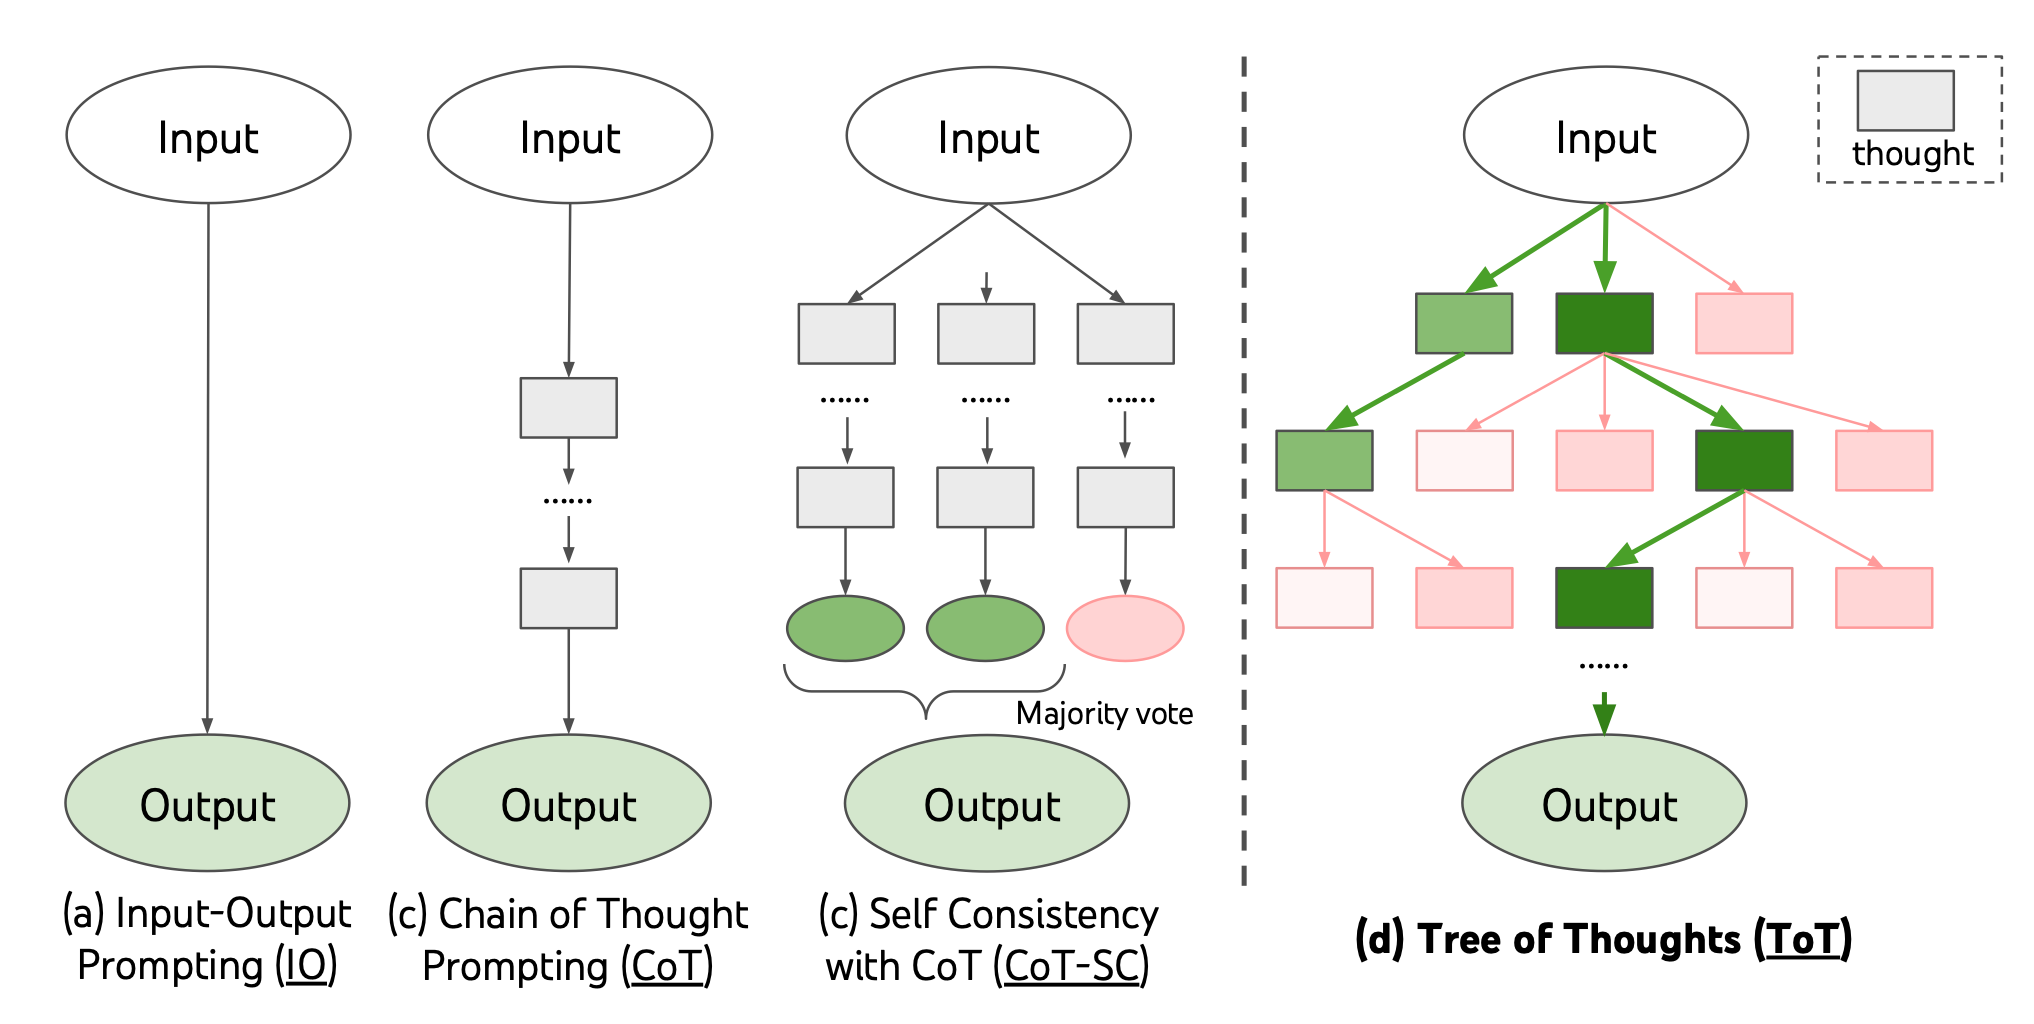
\includegraphics[width=\textwidth]{figures/tot}
    \end{figure}
\end{frame}

\begin{frame}
    {Tree of thought example}{}
    Branching, DFS/BFS, decide if the node is a deadend
    \begin{figure}
        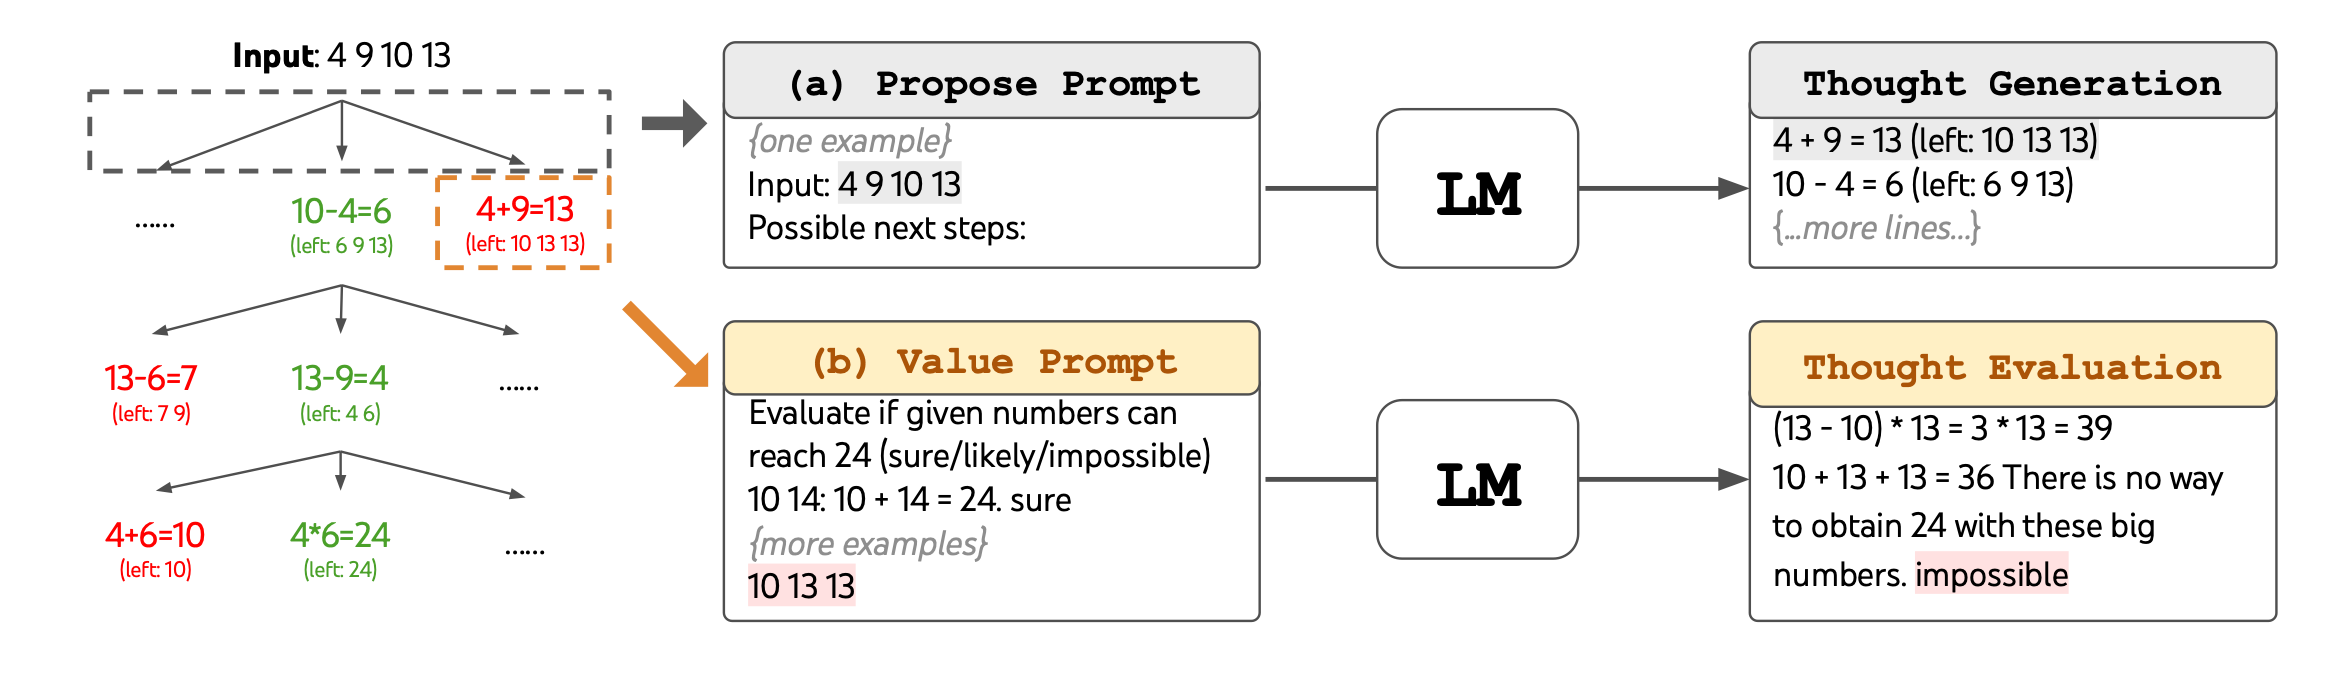
\includegraphics[width=\textwidth]{figures/tot-24}
    \end{figure}
\end{frame}

\begin{frame}
    {Summary}
    \begin{itemize}
        \itemsep1em
        \item Key challenge: align language with our intent (assisting with task X)
        \item Prompting: ``just ask'' the language model to do X
        \item Pros: simple and allows for creativity (ask for calibration, self-reflection)
        \item Cons: still an art rather than science (but can be made more reliable through finetuning)
    \end{itemize}
\end{frame}

\end{document}
